% Lines starting with a percent sign (%) are comments. LaTeX will 
% not process those lines. Similarly, everything after a percent 
% sign in a line is considered a comment. To produce a percent sign
% in the output, write \% (backslash followed by the percent sign). 
% ==================================================================
% Usage instructions:
% ------------------------------------------------------------------
% The file is heavily commented so that you know what the various
% commands do. Feel free to remove any comments you don't need from
% your own copy. When redistributing the example thesis file, please
% retain all the comments for the benefit of other thesis writers! 
% ==================================================================
% Compilation instructions: 
% ------------------------------------------------------------------
% Use pdflatex to compile! Input images are expected as PDF files.
% Example compilation:
% ------------------------------------------------------------------
% > pdflatex thesis-example.tex
% > bibtex thesis-example
% > pdflatex thesis-example.tex
% > pdflatex thesis-example.tex
% ------------------------------------------------------------------
% You need to run pdflatex multiple times so that all the cross-references
% are fixed. pdflatex will tell you if you need to re-run it (a warning
% will be issued)  
% ------------------------------------------------------------------
% Compilation has been tested to work in ukk.cs.hut.fi and kosh.hut.fi
% - if you have problems of missing .sty -files, then the local LaTeX
% environment does not have all the required packages installed.
% For example, when compiling in vipunen.hut.fi, you get an error that
% tikz.sty is missing - in this case you must either compile somewhere
% else, or you cannot use TikZ graphics in your thesis and must therefore
% remove or comment out the tikz package and all the tikz definitions. 
% ------------------------------------------------------------------

% General information
% ==================================================================
% Package documentation:
% 
% The comments often refer to package documentation. (Almost) all LaTeX
% packages have documentation accompanying them, so you can read the
% package documentation for further information. When a package 'xxx' is
% installed to your local LaTeX environment (the document compiles
% when you have \usepackage{xxx} and LaTeX does not complain), you can 
% find the documentation somewhere in the local LaTeX texmf directory
% hierarchy. In ukk.cs.hut.fi, this is /usr/texlive/2008/texmf-dist,
% and the documentation for the titlesec package (for example) can be 
% found at /usr/texlive/2008/texmf-dist/doc/latex/titlesec/titlesec.pdf.
% Most often the documentation is located as a PDF file in 
% /usr/texlive/2008/texmf-dist/doc/latex/xxx, where xxx is the package name; 
% however, documentation for TikZ is in
% /usr/texlive/2008/texmf-dist/doc/latex/generic/pgf/pgfmanual.pdf
% (this is because TikZ is a front-end for PGF, which is meant to be a 
% generic portable graphics format for LaTeX).
% You can try to look for the package manual using the ``find'' shell
% command in Linux machines; the find databases are up-to-date at least
% in ukk.cs.hut.fi. Just type ``find xxx'', where xxx is the package
% name, and you should find a documentation file.
% Note that in some packages, the documentation is in the DVI file
% format. In this case, you can copy the DVI file to your home directory,
% and convert it to PDF with the dvipdfm command (or you can read the
% DVI file directly with a DVI viewer).
% 
% If you can't find the documentation for a package, just try Googling
% for ``latex packagename''; most often you can get a direct link to the
% package manual in PDF format.
% ------------------------------------------------------------------


% Document class for the thesis is report
% ------------------------------------------------------------------
% You can change this but do so at your own risk - it may break other things.
% Note that the option pdftext is used for pdflatex; there is no
% pdflatex option. 
% ------------------------------------------------------------------
\documentclass[12pt,a4paper,oneside,pdftex]{report}

% The input files (tex files) are encoded with the latin-1 encoding 
% (ISO-8859-1 works). Change the latin1-option if you use UTF8 
% (at some point LaTeX did not work with UTF8, but I'm not sure
% what the current situation is) 
\usepackage[latin1]{inputenc}
% OT1 font encoding seems to work better than T1. Check the rendered
% PDF file to see if the fonts are encoded properly as vectors (instead
% of rendered bitmaps). You can do this by zooming very close to any letter 
% - if the letter is shown pixelated, you should change this setting 
% (try commenting out the entire line, for example).  
\usepackage[OT1]{fontenc}
% The babel package provides hyphenating instructions for LaTeX. Give
% the languages you wish to use in your thesis as options to the babel
% package (as shown below). You can remove any language you are not
% going to use.
% Examples of valid language codes: english (or USenglish), british, 
% finnish, swedish; and so on.
\usepackage[finnish,swedish,english]{babel}


% Font selection
% ------------------------------------------------------------------
% The default LaTeX font is a very good font for rendering your 
% thesis. It is a very professional font, which will always be 
% accepted. 
% If you, however, wish to spicen up your thesis, you can try out
% these font variants by uncommenting one of the following lines
% (or by finding another font package). The fonts shown here are 
% all fonts that you could use in your thesis (not too silly). 
% Changing the font causes the layouts to shift a bit; you many
% need to manually adjust some layouts. Check the warning messages
% LaTeX gives you.
% ------------------------------------------------------------------
% To find another font, check out the font catalogue from
% http://www.tug.dk/FontCatalogue/mathfonts.html
% This link points to the list of fonts that support maths, but
% that's a fairly important point for master's theses.
% ------------------------------------------------------------------
% <rant>
% Remember, there is no excuse to use Comic Sans, ever, in any
% situation! (Well, maybe in speech bubbles in comics, but there 
% are better options for those too)
% </rant>

% \usepackage{palatino}
% \usepackage{tgpagella}



% Optional packages
% ------------------------------------------------------------------
% Select those packages that you need for your thesis. You may delete
% or comment the rest.

% Natbib allows you to select the format of the bibliography references.
% The first example uses numbered citations: 
\usepackage[square,sort&compress,numbers]{natbib}
% The second example uses author-year citations.
% If you use author-year citations, change the bibliography style (below); 
% acm style does not work with author-year citations.
% Also, you should use \citet (cite in text) when you wish to refer
% to the author directly (\citet{blaablaa} said blaa blaa), and 
% \citep when you wish to refer similarly than with numbered citations
% (It has been said that blaa blaa~\citep{blaablaa}).
% \usepackage[square]{natbib}

% The alltt package provides an all-teletype environment that acts
% like verbatim but you can use LaTeX commands in it. Uncomment if 
% you want to use this environment. 
% \usepackage{alltt}

% The eurosym package provides a euro symbol. Use with \euro{}
\usepackage{eurosym} 

% Verbatim provides a standard teletype environment that renderes
% the text exactly as written in the tex file. Useful for code
% snippets (although you can also use the listings package to get
% automatic code formatting). 
\usepackage{verbatim}

% The listing package provides automatic code formatting utilities
% so that you can copy-paste code examples and have them rendered
% nicely. See the package documentation for details.
% \usepackage{listings}

% The fancuvrb package parovides fancier verbatim environments 
% (you can, for example, put borders around the verbatim text area
% and so on). See package for details.
% \usepackage{fancyvrb}

% Supertabular provides a tabular environment that can span multiple 
% pages. 
%\usepackage{supertabular}
% Longtable provides a tabular environment that can span multiple 
% pages. This is used in the example acronyms file. 
\usepackage{longtable}

% The fancyhdr package allows you to set your the page headers 
% manually, and allows you to add separator lines and so on. 
% Check the package documentation. 
% \usepackage{fancyhdr}

% Subfigure package allows you to use subfigures (i.e. many subfigures
% within one figure environment). These can have different labels and
% they are numbered automatically. Check the package documentation. 
\usepackage{subfigure}

% The titlesec package can be used to alter the look of the titles 
% of sections, chapters, and so on. This example uses the ``medium'' 
% package option which sets the titles to a medium size, making them
% a bit smaller than what is the default. You can fine-tune the 
% title fonts and sizes by using the package options. See the package
% documentation.
\usepackage[medium]{titlesec}

% The TikZ package allows you to create professional technical figures.
% The learning curve is quite steep, but it is definitely worth it if 
% you wish to have really good-looking technical figures. 
\usepackage{tikz}
% You also need to specify which TikZ libraries you use
\usetikzlibrary{positioning}
\usetikzlibrary{calc}
\usetikzlibrary{arrows}
\usetikzlibrary{decorations.pathmorphing,decorations.markings}
\usetikzlibrary{shapes}
\usetikzlibrary{patterns}


% The aalto-thesis package provides typesetting instructions for the
% standard master's thesis parts (abstracts, front page, and so on)
% Load this package second-to-last, just before the hyperref package.
% Options that you can use: 
%   mydraft - renders the thesis in draft mode. 
%             Do not use for the final version. 
%   doublenumbering - [optional] number the first pages of the thesis
%                     with roman numerals (i, ii, iii, ...); and start
%                     arabic numbering (1, 2, 3, ...) only on the 
%                     first page of the first chapter
%   twoinstructors  - changes the title of instructors to plural form
%   twosupervisors  - changes the title of supervisors to plural form
\usepackage[mydraft]{aalto-thesis}
%\usepackage[mydraft,doublenumbering]{aalto-thesis}
%\usepackage{aalto-thesis}


% Hyperref
% ------------------------------------------------------------------
% Hyperref creates links from URLs, for references, and creates a
% TOC in the PDF file.
% This package must be the last one you include, because it has
% compatibility issues with many other packages and it fixes
% those issues when it is loaded.   
\RequirePackage[pdftex]{hyperref}
% Setup hyperref so that links are clickable but do not look 
% different
\hypersetup{colorlinks=false,raiselinks=false,breaklinks=true}
\hypersetup{pdfborder={0 0 0}}
\hypersetup{bookmarksnumbered=true}
% The following line suggests the PDF reader that it should show the 
% first level of bookmarks opened in the hierarchical bookmark view. 
\hypersetup{bookmarksopen=true,bookmarksopenlevel=1}
% Hyperref can also set up the PDF metadata fields. These are
% set a bit later on, after the thesis setup.   


% Thesis setup
% ==================================================================
% Change these to fit your own thesis.
% \COMMAND always refers to the English version;
% \FCOMMAND refers to the Finnish version; and
% \SCOMMAND refers to the Swedish version.
% You may comment/remove those language variants that you do not use
% (but then you must not include the abstracts for that language)
% ------------------------------------------------------------------
% If you do not find the command for a text that is shown in the cover page or
% in the abstract texts, check the aalto-thesis.sty file and locate the text
% from there. 
% All the texts are configured in language-specific blocks (lots of commands
% that look like this: \renewcommand{\ATCITY}{Espoo}.
% You can just fix the texts there. Just remember to check all the language
% variants you use (they are all there in the same place). 
% ------------------------------------------------------------------
\newcommand{\TITLE}{Clustering of Finnish scientific publications 
by discipline}
\newcommand{\FTITLE}{Suomalaisten tieteellisten julkaisujen 
ryhmittely
tieteenaloittain klusteroimalla}
\newcommand{\STITLE}{Klustring av finl�ndska vetenskapliga 
publikationer efter disciplin}
\newcommand{\SUBTITLE}{No subtitle}
\newcommand{\FSUBTITLE}{Ei alaotsikkoa}
\newcommand{\SSUBTITLE}{Igen undertitel}
\newcommand{\DATE}{November 30, 2017}
\newcommand{\FDATE}{30. marraskuuta 2017}
\newcommand{\SDATE}{Den 30 November 2017}

% Supervisors and instructors
% ------------------------------------------------------------------
% If you have two supervisors, write both names here, separate them with a 
% double-backslash (see below for an example)
% Also remember to add the package option ``twosupervisors'' or
% ``twoinstructors'' to the aalto-thesis package so that the titles are in
% plural.
% Example of one supervisor:
%\newcommand{\SUPERVISOR}{Professor Antti Yl�-J��ski}
%\newcommand{\FSUPERVISOR}{Professori Antti Yl�-J��ski}
%\newcommand{\SSUPERVISOR}{Professor Antti Yl�-J��ski}
% Example of twosupervisors:
\newcommand{\SUPERVISOR}{Professor Samuel Kaski}
\newcommand{\FSUPERVISOR}{Professori Samuel Kaski}
\newcommand{\SSUPERVISOR}{Professor Samuel Kaski}

% If you have only one instructor, just write one name here
\newcommand{\INSTRUCTOR}{Yrj� Leino Lic.Sc. (Tech.)}
\newcommand{\FINSTRUCTOR}{Tekniikan lisensiaatti Yrj� Leino}
\newcommand{\SINSTRUCTOR}{Teknologie licentiat Yrj� Leino}
% If you have two instructors, separate them with \\ to create linefeeds
% \newcommand{\INSTRUCTOR}{Olli Ohjaaja M.Sc. (Tech.)\\
%  Elli Opas M.Sc. (Tech)}
%\newcommand{\FINSTRUCTOR}{Diplomi-insin��ri Olli Ohjaaja\\
%  Diplomi-insin��ri Elli Opas}
%\newcommand{\SINSTRUCTOR}{Diplomingenj�r Olli Ohjaaja\\
%  Diplomingenj�r Elli Opas}

% If you have two supervisors, it is common to write the schools
% of the supervisors in the cover page. If the following command is defined,
% then the supervisor names shown here are printed in the cover page. Otherwise,
% the supervisor names defined above are used.
%\newcommand{\COVERSUPERVISOR}{Professor Antti Yl�-J��ski, Aalto 
%University\\
%  Professor Pekka Perustieteilij�, University of Helsinki}

% The same option is for the instructors, if you have multiple instructors.
% \newcommand{\COVERINSTRUCTOR}{Olli Ohjaaja M.Sc. (Tech.), Aalto University\\
%  Elli Opas M.Sc. (Tech), Aalto SCI}


% Other stuff
% ------------------------------------------------------------------
\newcommand{\PROFESSORSHIP}{Computer Science}
\newcommand{\FPROFESSORSHIP}{Tietojenk�sittelytiede}
\newcommand{\SPROFESSORSHIP}{Datavetenskap}
% Professorship code is the same in all languages
\newcommand{\PROFCODE}{SCI3042}
\newcommand{\KEYWORDS}{clustering, bibliomterics}
\newcommand{\FKEYWORDS}{ryv�stys, bibliometriikka}
\newcommand{\SKEYWORDS}{klusteranalys, bibliometri}
\newcommand{\LANGUAGE}{English}
\newcommand{\FLANGUAGE}{Englanti}
\newcommand{\SLANGUAGE}{Engelska}

% Author is the same for all languages
\newcommand{\AUTHOR}{Juho Lehtonen}


% Currently the English versions are used for the PDF file metadata
% Set the PDF title
\hypersetup{pdftitle={\TITLE\ \SUBTITLE}}
% Set the PDF author
\hypersetup{pdfauthor={\AUTHOR}}
% Set the PDF keywords
\hypersetup{pdfkeywords={\KEYWORDS}}
% Set the PDF subject
\hypersetup{pdfsubject={Master's Thesis}}


% Layout settings
% ------------------------------------------------------------------

% When you write in English, you should use the standard LaTeX 
% paragraph formatting: paragraphs are indented, and there is no 
% space between paragraphs.
% When writing in Finnish, we often use no indentation in the
% beginning of the paragraph, and there is some space between the 
% paragraphs. 

% If you write your thesis Finnish, uncomment these lines; if 
% you write in English, leave these lines commented! 
% \setlength{\parindent}{0pt}
% \setlength{\parskip}{1ex}

% Use this to control how much space there is between each line of text.
% 1 is normal (no extra space), 1.3 is about one-half more space, and
% 1.6 is about double line spacing.  
% \linespread{1} % This is the default
% \linespread{1.3}

% Bibliography style
% acm style gives you a basic reference style. It works only with numbered
% references.
\bibliographystyle{acm}
% Plainnat is a plain style that works with both numbered and name citations.
% \bibliographystyle{plainnat}


% Extra hyphenation settings
% ------------------------------------------------------------------
% You can list here all the files that are not hyphenated correctly.
% You can provide many \hyphenation commands and/or separate each word
% with a space inside a single command. Put hyphens in the places where
% a word can be hyphenated.
% Note that (by default) LaTeX will not hyphenate words that already
% have a hyphen in them (for example, if you write ``structure-modification 
% operation'', the word structure-modification will never be hyphenated).
% You need a special package to hyphenate those words.
\hyphenation{di-gi-taa-li-sta yksi-suun-tai-sta}



% The preamble ends here, and the document begins. 
% Place all formatting commands and such before this line.
% ------------------------------------------------------------------
\begin{document}
% This command adds a PDF bookmark to the cover page. You may leave
% it out if you don't like it...
\pdfbookmark[0]{Cover page}{bookmark.0.cover}
% This command is defined in aalto-thesis.sty. It controls the page 
% numbering based on whether the doublenumbering option is specified
\startcoverpage

% Cover page
% ------------------------------------------------------------------
% Options: finnish, english, and swedish
% These control in which language the cover-page information is shown
\coverpage{english}


% Abstracts
% ------------------------------------------------------------------
% Include an abstract in the language that the thesis is written in,
% and if your native language is Finnish or Swedish, one in that language.

% Abstract in English
% ------------------------------------------------------------------
\thesisabstract{english}{
\fixme{Abstract text here.} 
% Fixme is a command that helps you identify parts of your thesis that still
% require some work. When compiled in the custom \texttt{mydraft} mode, text
% parts tagged with fixmes are shown in bold and with fixme tags around them. When
% compiled in normal mode, the fixme-tagged text is shown normally (without
% special formatting). The draft mode also causes the ``Draft'' text to appear on
% the front page, alongside with the document compilation date. The custom
% \texttt{mydraft} mode is selected by the \texttt{mydraft} option given for the
% package \texttt{aalto-thesis}, near the top of the \texttt{thesis-example.tex}
% file.
}

% Abstract in Finnish
% ------------------------------------------------------------------
\thesisabstract{finnish}{
Suomekielinen tiivistelm�
}

% Abstract in Swedish
% ------------------------------------------------------------------
\thesisabstract{swedish}{
Svensk text h�r.
}


% Acknowledgements
% ------------------------------------------------------------------
% Select the language you use in your acknowledgements
\selectlanguage{english}

% Uncomment this line if you wish acknoledgements to appear in the 
% table of contents
%\addcontentsline{toc}{chapter}{Acknowledgements}

% The star means that the chapter isn't numbered and does not 
% show up in the TOC
\chapter*{Acknowledgements}

Some acknowledgements here...

Thank you...
\vskip 10mm

\noindent Espoo, \DATE
\vskip 5mm
\noindent\AUTHOR

% Acronyms
% ------------------------------------------------------------------
% Use \cleardoublepage so that IF two-sided printing is used 
% (which is not often for masters theses), then the pages will still
% start correctly on the right-hand side.
\cleardoublepage
% Example acronyms are placed in a separate file, acronyms.tex
\addcontentsline{toc}{chapter}{Abbreviations and Acronyms}
\chapter*{Abbreviations and Acronyms}

% The longtable environment should break the table properly to multiple pages, 
% if needed

\noindent
\begin{longtable}{@{}p{0.25\textwidth}p{0.7\textwidth}@{}}
LSA & Latent semantic analysis \\
MDS & Multi-dimensional scaling \\
SVD & Singular value decomposition \\
tf-idf & term frequency-inverse document frequency \\
note & Note also, that this list is not compulsory, and should be 
omitted if you have only few abbreviations \\

\end{longtable}


% Table of contents
% ------------------------------------------------------------------
\cleardoublepage
% This command adds a PDF bookmark that links to the contents.
% You can use \addcontentsline{} as well, but that also adds contents
% entry to the table of contents, which is kind of redundant.
% The text ``Contents'' is shown in the PDF bookmark. 
\pdfbookmark[0]{Contents}{bookmark.0.contents}
\tableofcontents

% List of tables
% ------------------------------------------------------------------
% You only need a list of tables for your thesis if you have very 
% many tables. If you do, uncomment the following two lines.
% \cleardoublepage
% \listoftables

% Table of figures
% ------------------------------------------------------------------
% You only need a list of figures for your thesis if you have very 
% many figures. If you do, uncomment the following two lines.
% \cleardoublepage
% \listoffigures

% The following label is used for counting the prelude pages
\label{pages-prelude}
\cleardoublepage

%%%%%%%%%%%%%%%%% The main content starts here %%%%%%%%%%%%%%%%%%%%%
% ------------------------------------------------------------------
% This command is defined in aalto-thesis.sty. It controls the page 
% numbering based on whether the doublenumbering option is specified
\startfirstchapter

% Add headings to pages (the chapter title is shown)
\pagestyle{headings}

% The contents of the thesis are separated to their own files.
% Edit the content in these files, rename them as necessary.
% ------------------------------------------------------------------
\chapter{Introduction}
\label{chapter:intro}
% The target
% ==========
This thesis handles the problem of clustering Finnish scientific 
publications by their metadata. The target is to cluster 
them as well as possible by their scientific discipline. \fixme{
Tahan enemman tavoitteen kuvausta ei viela maarittelyn vaikeutta.}
Of course 
the ``wellness'' of a clustering measured by how it fits to 
scientific fields is a tricky issue for at least couple of 
reasons.


% Obstacles
% =========
First, there is no general consensus about what is the correct 
partition of all science to different branches. It might be depend 
on specific need or individual opinion where the line between two 
related discipline lies.

Second, science is evolving all the time. What was yesterday seen 
simply as chemistry could today be viewed as organic and inorganic 
chemistry.

Third, the definition of scientific disciplines depends also how 
closely we look into a topic. Sometimes chemistry is sufficent 
description for eg. a publication and sometimes we need to define 
it more accurately as organic chemistry.
% LMa: Tahan maininta poikkitieteellisten alojen 
% ongelmallisuudesta, onko bioinformatiikka, biologiaa, 
% tietotekniikkaa vai oma tieteenalansa.

But despite this ambiguousness of the target we define and 
justify some goals and how to measure our success.


% Environment/background
% ======================
In Finland there are 15 universities and 23(+2) universities of 
applied sciences. Additionally there are 12 research institutes.
Each year Finnish scientific efforts produce about 
10000 publications in all scientific disciplines. 
\fixme{10000 tulee siis WOS ja Elsevierilta} The Ministry of 
Education and Culture oversees what is researched and in what 
quanities in the Finnish research.
Classifying articles by discipline enables different types of 
bibliometric analysis.
% It is also ill posed problem because there is no one right answer
% for the problem. Different tasks require different classification.
Because of the amount of the scientific articles manual 
classification is not applicable. \fixme{Also: kukaan tuskin 
pystyy hallitsemaan kaikkia tieteenaloja. Tavoitteena tyokalu, 
jolla analyysin tekija voi luokitella }
% All these are manual methods. Automatic methods are needed...
Automatic methods should be able to label the article by some 
criterion to the (subjectively) obvious discipline. The input for 
automatic method can usually at most be the whole article and 
perhaps some metadata describing it. The metadata can be 
created by the author or the publisher or some archive.

\fixme{What methods used?}
Different methods have been suggested. NN1 suggested SOME METHOD. 
NN2 suggested SOME OTHER METHOD. NN3 suggested YET A METHOD.

In this thesis we will try to cluster Finnish publications by 
discipline by using the metadata.





\section{Problem statement}

Refactor from above...

\section{Structure of the Thesis}
\label{section:structure} 

% Use transition in your text, meaning that you should help
% the reader follow the thesis outline. Here, you tell what will be in
% each chapter of your thesis.
In chapter 2. we will shortly present the background...


\chapter{Background}
\label{chapter:background}

% Tiedonhankintaa suunnitellessasi voi miettiä vastauksia mm. 
% seuraaviin aiheen määrittelyä selventäviin tutkimuskysymyksiin:
% 
%     Mistä aiheesta tietoa tarvitaan?
%       bibliometriikasta, sen määritelmästä sekä klusteroinnista
%     Mihin tarkoitukseen tietoa tarvitaan?
%       Aiheen taustan kuvailuun, menetelmien kuvailuun ja 
%       valitun menetelmän toteuttamiseen
%     Mikä aiheessa on keskeistä?
%       Klusterointimenetelmän kokeilu ja tulosten raportointi
%     Mistä näkökulmasta aihetta lähestytään?
%       Käytännön implementaation kokeilulla
%     Mitä aiheesta tiedetään jo ennalta?
%       Klusteroinnista perusteet, bibliometriikasta vähemmän
%     Tarvitaanko yleis- vai tieteellistä tietoa?
%       Bibliometriikasta tarvitaan vähän yleistietoa, 
%       klusteroinnista tieteellistä.
%     Tarvitaanko kuva-aineistoa?
%       Ei muuta kuin itse tuotetut
%     Minkä ikäistä tietoa tarvitaan?
%       Yleis- ja taustatiedot vanhoista asioista, aiheen 
%       oleellinen tieto uusinta
%     Minkä kielistä tietoa tarvitaan?
%       suomi ja englanti käy


In this chapter we briefly introduce clustering and how it is 
positioned in the larger field of machine learning. But first we
describe what bibliometrics is.
% Taman esittelyjarjestyksen voi vaihtaa myohemmin

\section{Bibliometrics}
\label{sec:bibliometrics}
% Mita bibliometriikka on?
% Valmis --->-v
Bibliometrics is a study of written scientific records. The 
records may be books, articles, letters in scientific journals, 
conference papers and so on. Bibliometrics studies how these 
products of research are communicated, how are they related to 
each other, what kind of properties they have and what can be 
learned about the science in general by analysing them.

% Mihin bibliometriikka pyrkii vastaamaan?
Bibliometrics seeks to answer questions like ``How many 
publications has an author authored?'', ``How many citations an 
author has'', ``What are the 
cited publications of a scientific document?''. It also studies
a bit more boarder questions like ``How many publications
on discipline X been published a year?'', ``Which research area
does this publication belong to?'', ``What other publications 
belong to this research area?'', ``When has this research area
emerged?'', ``What are the most important related research areas
of this discipline?'' an so on.

% Background/history
% ==================
% Mika bibliometriikan historia on?
% OK --->-v
Classifying things is often the first thing we do when we observe 
the world. On the other hand, counting the frequenzies of objects
and comparing these numbers often helps to put things in 
perspective.
% Tahan voisi laittaa sidontaa todennakoisyyslaskennalla tjsp.
One of the earliest studies that is generally considered
bibliometrics was Cole's and Eales' analysis to the anatomy 
literature in 1917 \cite{cole_history_1917}. In this study they 
researched the anatomy literature from 1543 through 1860 with the 
intention to graph the growth of of the number of documents over 
the three centuries, to present ``the performance'' of each 
European country, to observe the most popular topics among 
scholars from time to time, and to compare the advancement and 
devolution stages of the research with different societal 
events \cite{bellis_bibliometrics_2009}.
As the number of scientific publications has enormously increased
the need to automatically analyze them has become apparent.
The basic analysis on top of which more detailed studies can be 
built on is classifying each publication to research areas and
disciplines.
% The need for some kind of bibliometric indices rise in the 
% First modern(?) classification was... by... some 
% indexing/publishing/to facilitate communication...
% At some point more and more automation was needed for bibliomterics
% There has been lot of study in automatically classificating the 
% science. 


\subsection{Classification in bibliometrics}
% Specific charasteristics of classifying the bibliometrics
% Miten bibliometriikkaa voidaan jasentaa / mista se koostuu?
% Existing classification systems / methods
% =========================================
\fixme{Onko Scopus tässä relevantti jos ei Scopus-dataa?}
Currently, the most popular systems to classify the publications 
into research areas are the Clarivate's (formerly Thomson Reuters)
Web of Science and Elsevier's Scopus classification
systems. These classification systems classify the journals into
one or more research areas. \cite{waltman_new_2012} Publications
are then classified to research areas based on in which journal they
were published. WoS uses approximately 250 \emph{subject categories}
in its classification. Each journal can belong 
to one or up to six categories. The categories have been created
at least or before early 1960's by manually classifying journals.
New journals were added one at the time after visual inspection of
citation information. New categories were added when when old ones
grew \cite{pudovkin_algorithmic_2002}. As for Scopus, according to 
Wang and Waltman \cite{wang_large-scale_2016}, ``there seems to be no 
information at all on the construction of its classification 
system''.

Also an independent journal level classification system has been 
developed. \cite{archambault_towards_2011}
Journal level classification systems have known limitations.
They are, for example, unable to meaningfully classify
publications published in multidiscipline journals.
Also some discipline specific classification systems exists such 
as (check them...).
An alternative classification system is publication level 
classification where each publication is classified based on some 
information extracted directly from the publication self such as
words used in the title and/or abstract, keywords attached by the
authors or publisher or citations to other publications.
Shu et al. have compared journal and paper level classification
approaches and found that publication level classification could
provide better classification \cite{shu_comparing_2019}.
% Usually classification of publications or journals can be approached 
% at least from multiple directions. There is clustering based method,
% the network based method and the combination of the two.
% In the network method

% ACM:n luokittelujärjestelmä esimerkkinä? CLSF?...
Bibliometric research 
uses mainly three types of methods; citation based, text analysis 
based or combination of the two \cite{janssens_hybrid_2009}.
Citation based methods study citations of publications and produce
networks where publications are nodes connected by citations as 
edges. In
 the rare case of publication having a direct quote including a
 citation, the citation is not counted unless it is also a
 citation of the publication itself.
Connection between two publications can be 
formed by a direct citation, bibliometric coupling where 
publications are connected when a third publication cites them 
both or co-citations where publications are connected if they 
cite the same third publication.

Text analysis based methods examine the title, the abstract or 
the whole text content of the publication itself and classify 
the publications or journals by the topic model created 
\cite{blei_latent_2003}.
Hybrid models combine both approaches. Authors and their
affilations are not used in this work because we cannot uniquely
identify them and we can't assume their field of science that is
our interest here.

% Tama on kompelosti ilmaistu, korjaa
% Verkkoanalyysin nakokulma
% These research products and relations between them form a 
% network that can reveal something about the structure of 
% different scientific disciplines. Finding the structure of this 
% kind of data set is called classification or clustering.


% Previous results using clustering bibliometrics
% ===============================================
% Kirjoitettu yllä olevaan


\subsection{Bibliometrics in Finland}
Ministry of Education and Culture of Finland provides yearly
updated bibliometric analyses of Finnish research activities 
based on both Web Of Science citation index 
and Elsevier's Scopus database \cite[Vipunen 
service]{noauthor_ministry_2019}. The corresponding source 
system classification for a field of science is used and
aggregated to match the Statistics Finland classification 
\cite{auranen_tieteen_2018}. CSC - 
IT Center for Science is responsible of the actual technical 
implementation of the service.

One of the earlier and comprehensive bibliometric research of 
Finnish science is a report by Persson et al. 
\cite{persson_bibliometric_2000} which mapped the situation and 
development of Finnish science 1981-1998.
This, however, is a report which concentrates on bibliometric 
analysis based on the map of science provided by WoS subject 
categories. But if we want to explore how the Finnish scientific 
disciplines themselves have evolved over time these pre-defined 
subject categories are quite rigid framework. For that reason we 
want to experiment creating an alternative mapping of science by 
clustering. 

So, as opposed to bibliometric analyses seeking to understand the
state of a scientific discipline as defined by some existing 
definition, we want to experiment/inspect how to define 
scientific disciplines to be used in bibliometric analyses.

%Efforts to cluster Finnish research include a study by...

Suominen and Toivanen used unsupervised learning-based topic 
modeling to create a map of science for Finnish publications from 
1995-2011. They evaluated it by comparing the results with WoS 
based classification and concluded that superiority of the method
depends on the purpose of analysis. Traditional manually created 
classifications are relevant for information retrieval while 
machine learning methods can reveal new emerging areas of science 
\cite{suominen_map_2016}. Compared to our work here, their 
analysis method topic modeling differs from hierarchical 
clustering albeit both are unsupervised learning methods.
\fixme{Vie myös ``Discussion'' -osioon.}

Our research question here is: "How to automatically cluster 
Finnish scientific publications and how does that clustering 
compare to existing fiels of science classification by WoS?" We 
will use hierarchical clustering on features derived from titles,
abstracts and keywords in publication metadata.


\section{Clustering}
The methods discussed in this work belong to the field of machine 
learnig. The field has it's roots in statistics and engineering 
and is itself part of artificial intelligence.
The methods in machine learnig can be divided to supervised, 
unsupervised and reinforced learning \cite{alpaydin2004introduction}.

Commonly for all methods we define $X$ as
the sample data and $Y$ as label indicating which class our data 
sample $X$ belongs. We also have to choose the model $f()$ for
learning from the data. Then we can state our learning problem as
a function $Y = f(w \cdot X)$, where $w$ is a weight vector, 
which would give a prediction of the class $Y$ of the sample data
$X$. 
Assuming we have enough of samples $X$ we then teach our model 
with training data. That is, we solve the weights $w$ using the
loss function such that it optimizes the difference between the 
true and predicted class labesl $Y$.

Supervised learnig methods include classification and continuous 
estimation (regression)
where the class of the training samples, or the target values in 
case of regression, $Y$ is known. Example of a classification 
problem is optical character recognition where the system is 
taught with example of characters along with their correct labels.

For unsupervised learning the correct answer or the label $Y$ is not known. 
Instead a model is applied such that it finds regularities in the
input data $X$. Example of unsupervised learning problem is 
finding anomalities that don't fit in the group, such as analysing
log files of a computer system to find a possible intruder.

Unsupervised learning methods include clustering, dimensionality
reduction and topic modeling for instance. Clustering try to 
distinguish patterns in the data and discriminate unrelated 
objects into separate clusters and aggregate related objects into
same cluster.

In reinforced learning we want the system to learn a sequence of
actions leading to desired outcome. For example we may want the 
system to learn to win a game. In that case individual actions
are not important but the end result as there are many ways to win
a game. So the system repaeatedly tries different combinations of
actions while it receives the result of it's combined actions.

\subsubsection{Model selection}
Generally all machine learning problems are ill-posed in the sense 
that a unique solution for the problem can't be found unless some
assumptions, or \emph(inductive bias), are introduced. This begins 
with selecting the learning algorithm.

Here we will unsupervised learning to shape a mapping of 
scientific disciplines because we want to learn the possible 
intristic structure of sciencetific knowledge. We will use 
clustering because it's quite simple and familiar to us. 
There are many different clustering algorithms from which to 
choose. Some often used common algorithms are k-means, hierarchical
clustering, density based scan clustering and Gaussian clustering.
We will use hierarchical clustering. Among the hierarchical 
clustering there are yet different parameters to choose. 
clustering as our method because clustering methods with different linkages applied 
to search query results are experimented by Korenius et al. 
\cite{korenius_hierarchical_2006}.

\fixme{Ero verkkoanalyysiin: lyhyesti}


\subsection{Choosing the number of clusters}
\fixme{Yleisellä tasolla: "tämän tyyppisiä menetelmiä on 
olemassa", "ne soveltuvat tähän ja tähän käyttötarkoitukseen". 
Helppo löytää ja käyttää viitteitä; esim. käytetty siinä ja siinä, 
meta- ja review-tutkimukset}
% 29.4.2020 Lyhyesti vain

In hierarchical clustering number of clusters can be chosen after 
the data has been clustered and the dendogram \fixme{explain more}
 formed.
\fixme{citation} By 
looking the dendrogram and using different metrics the number of 
clusters can be chosen.


\subsection{Evaluating of clustering results}
We will use Calinski \& Harabazt criterion (or the variance ratio 
criterion (VRC)) as an evaluation criterion for 
deciding the number clusters \cite{calinski_dendrite_1974}. It 
is defined as
\begin{equation}
 VRC_k = \frac{SS_B}{N-k} \frac{SS_W}{k-1},
\end{equation}
where $SS_B$ is the overall variance between clusters, $SS_W$ is 
the over variance within clusters, $k$ is the number of clusters 
and $N$ is the number of observations.

The overall variance between clusters $SS_B$ is defined as
\begin{equation}
 SS_B = \sum_{i=1}^k n_i ||m_i-m||^2,
\end{equation}
where $k$ is the number of clusters, $n_i$ is the number of 
observations in cluster $i$, $m_i$ is centroid of cluster $i$, 
$m$ is the overall mean of the sample data and $||m_i-m||$ is the 
Euclidean distance between the two vectors.

The overall variance within clusters $SS_W$ is defined as
\begin{equation}
 SS_W = \sum_{i=1}^k \sum_{x\in c_i} ||x-m_i||^2,
\end{equation}
where $k$ is the number of clusters, $x$ is the oservation, 
$c_i$ is the $i$th cluster, $m_i$ is centroid of cluster $i$, and 
$||x-m_i||$ is the Euclidean distance between the two vectors.
The larger the Calinski \& Harabazt criterion, the better the 
cluster structure.
\fixme{Tämä suoraan: 
https://www.mathworks.com/help/stats/clustering.evaluation.calinsk
iharabaszevaluation-class.html pitäisikö kertoa ``omin sanoin''?}



\subsubsection{Manually annotated validation set}
% Gold standard set. Actually a gold standard set would be a set
% of all data sets with abstract excluding sets that don't have it.
We will create a manually annotated validation set for calculating
precision, recall and metrics derived from those.
% määrittele peruskäsitteet kuten precision ja recall
The validation
set consists of $500$ publications from three different fields of
science, two more similar sub fields of computer science, 
information systems and artificial intelligence, and one more
distant from those, clinical neurology.

Publications are inspected by title, abstract, keywords, journal
and publisher assigned disciplines of the journal. We checked 
just by layman's reasoning if the labeled discipline seemed 
plausible. Because of the journal based 
classification, most publications had more than one 
assigned discipline. Only discipline labels named 
previously were retained because we were wanted test 
how well our clustering method separated these three 
groups regardless their labels. So essentially the 
labels could have been eg. 1, 2, 3. Publications
with critically missing data, unclear discipline assignment and
heavily applied publications were excluded from validation set.
Goal was to achieve evaluation measurements based on a quite 
clearly separated set of publications. More vaguely classifiable
publications were included for comparison. We asked an another 
opinion for publications that could have been in more 
than one of our categories. For manually curated validation set 
with discipline assignment and justifications for
possible exclusion see appendix (Insert reference!).

The basic problem is that fields of science can not be 
defined so that they clearly differ from each other. Where one 
discipline end the other has already started like metallurgy and 
material science. Likewise, there are lots of publications that 
handle topics belonging to more than one discipline, eg. this 
thesis discusses clustering and bibliometrics. So when annotating 
publications, deciding if a publication belonged to
a discipline or not felt often quite difficult. Often the 
separation between disciplines felt quite arbitrary. For example
an article describing using wavelet transformation for coding noisy
images was decided to belong to CS information systems whereas an
article describing wavelet based corner detection using SVD was
decided to belong to CS artificial intelligence.
For CS artificial intelligence we mostly selected publications 
which
mentioned some dimensionalty reduction or machine learning related
term or concept.
CS information systems ended up being quite like some ``others'' 
or
``the rest'' dump class. It would have publications such as
``A reference model for conceptualising the convergence of 
telecommunications and datacommunications service platforms'',
``Developing a distributed meeting service to support mobile 
meeting participants'',
``On voice quality of IP voice over GPRS'',
\fixme{Perustele vain yhteen alaan luokittelu. ``Tukeudun 
WOS-luokitteluun''.}
\fixme{Selvennä yläluokka-alaluokka-jako: CS general vs. CS 
information system tai CS artificial intelligence.}


%\chapter{Bibliometric}
\label{chapter:environment}

A problem instance is rarely totally independent of its environment.
Most often you need to describe the environment you work in, what
limits there are and so on. This is a good place to do that. First we
tell you about the LaTeX working environments and then is an example
from an thesis written some years ago.


\section{Clustering}
\label{sec:environments}



\subsection{Environment}







\chapter{Methods}
\label{chapter:methods}
In this chapter we present the methods used in the clustering. We 
follow the logical order the methods are applied on data.

\section{SVD}
\label{sec:svd}
There are multiple ways to use input metadata of the publications; 
put all text to one bin and use text analysis methods to that. 
Alternatively we could assume different distribution for each 
metadata field and treat them separately.

\section{Agglomerative clustering}
\label{sec:agglomerativeclustering}
There are also multiple methods to use for the problem. LDA is one.

\subsection{Distance metric}
Data is high dimensional so choosing distance measure is 
important. The higher the number of dimensions the more similar 
distance each observation is from every other observation. This 
known as \emph{curse of dimensionality} \fixme{citation}.
Possible distance measures are:
- cosine angle (uncentered Pearson correlation)\fixme{look: 
\url{https://www.researchgate.net/post/What_is_the_best_distance_
measure_for_high_dimensional_data/4}}
-euclidean
-mahalnobis

\subsection{Linkage methods}
In this work we use agglomerative hierarchical clustering with 
Ward's distance metric.\fixme{citation}

\subsubsection{Single linkage}
\subsubsection{Complete linkage}
\subsubsection{Average linkage}
\subsubsection{Ward's method}

\subsection{Complexity}
Time and space requirements of used agglomerative clustering method
are $O(N^2)$ for both.\fixme{citation}



 
\chapter{Implementation}
\label{chapter:implementation}
Here we describe how the methods are implemented to achieve the 
clustering. First we describe how the raw text data is 
pre-processed 

We implemented a workflow for clustering using Python's 
scikit-learn package. \fixme{Include a graph visualizing the 
workflow.}

First data was read from raw files obtained from publishers. 
%(Actually YL probably also preprocessed data before passing it 
% to me.)
Unrelevant metadata fields were omitted and the relevant were read 
into a dictionary. We choose to keep title, abstract and keyword
fields. Terms in keyword fields were concatenated to combined 
terms: ``allergic\_contact\_dermatitis''. Another option would be to
count n-grams to preserve the meaning of combined terms. (Justify 
decision.) Title and abstract fields were treated with a bag of 
words representation. (Explain.)



Data was lemmatized. We choose to remove all plain numbers from
data. Another option is to replace numbers with dummy '\#NUMBER'.
That could help separate natural sciences from humanities. Because 
we didn't have proper knowledge on the issue removal was chosen. So 
numbers would be ignored. That would be a more neutral way to treat 
them. (How? Explain...)

Running preliminary tests for 2000 publications with tf-idf's maximum and 
minimum document frequencies set to $max_df=0.5$ 
and $min_df=2$ (integers denote absolute count value) respectively
resulted a feature space of 3372 terms and a stop word list of 7475 
terms. The stop word list included 352 a priori set words and words
that occurred in too many ($max_df$) or too few ($min_df$) 
documents. Terms that were filtered out as too frequent or too few
were for example: ``haemoglobin\_a'', ``jacobian\_matrix'', 
``parthenogenetic'', ``chelation\_by\_saccharide\_molecules'', 
``leg\_blood\_supply'', ``computational\_fluid\_dynamics'', 
``pigment'', ``hdtv'', ``nicotinic\_receptor''.

(Interesting would be to know the frequencies of the filtered-out 
terms. It didn't come out straight from TfIdfVectroizer class used 
but taking different levels of $min_df$ and $max_df$ could be used 
to view different frequency groups.)

When trying with $max_df=0.6$ we get feature space of XXXX and 
YYYY stop words.



\chapter{Evaluation}
\label{chapter:evaluation}

We need some sort of tool to measure the ``goodness'' of the 
clustering. As we work with text data the dimesionality increases 
quite high and projecting data down to 2 or 3 dimensions for 
visualization is not a simple task. (We come back to visualization 
later though.)
So we have to resort to measurements derived from the 
resulting clustering itself. If we knew some underlying ground 
truth behind our clustering problem we could validate our result 
against it. But as mentioned earlier, even defining what actually 
are the current fields of science depends on who you ask and for 
what purpose the definition is needed. So the the ground truth 
here is only one measure for our results.
In the lack of ground truth we can use some ``internal'' goodness 
measure for the resulting clustering. These kind of measures 
basically try to infer how dense the clusters are compared to how 
sparse the inter-cluster space is and how well the clusters are 
separated from each other.
One such measure to estimate the ``goodness'' of a clustering is 
silhouettes. Silhoutettes use average proximities which are know 
to work best with clear, compact and spherical clusters 
\cite{rousseeuw_silhouettes:_1987}. Silhouette value for an item 
is defined as:

Silhoutte values for 6000 publications clustered with 
agglomerative clustering with Ward's method, number of clusters 
64, are seen in Figure~\ref{fig:silh01}.
\begin{figure}[ht]
  \begin{center}    
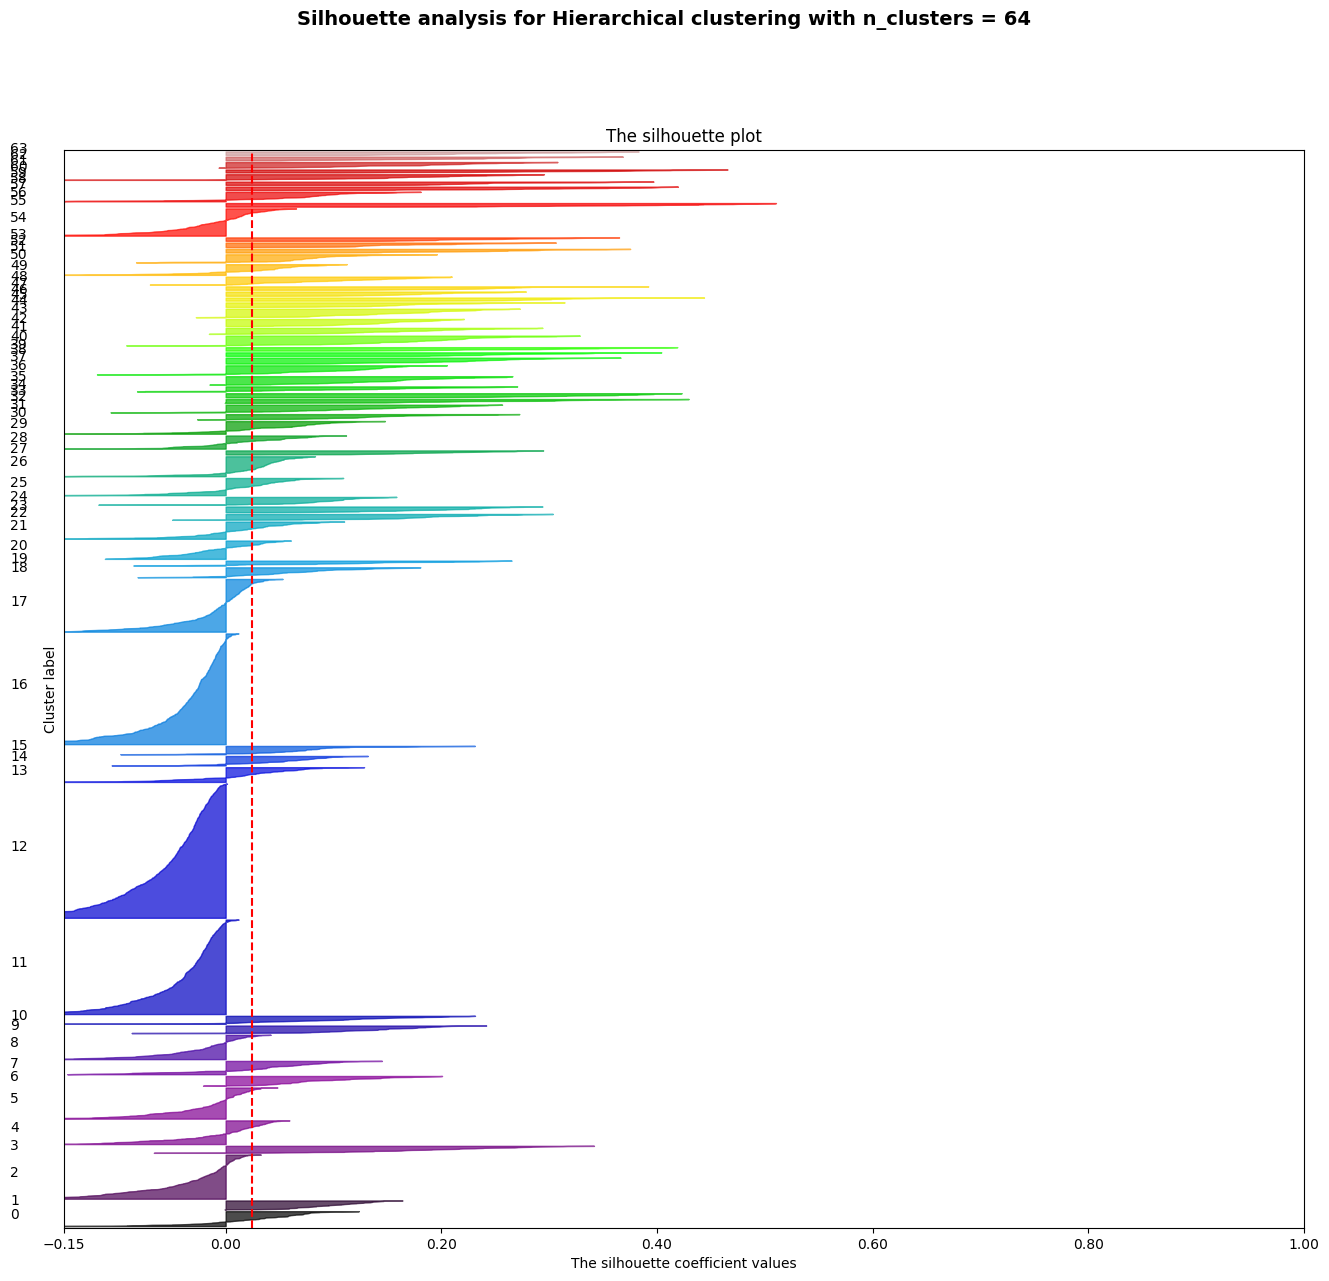
\includegraphics[width=13cm]{images/6000-64-400-Hierarchical-silhouette-plot.png}
    \caption{Silhoutte values of 6000 items clustered with 
    agglomerative clustering with Wrad's method, 64 clusters, 
    LSA with 400 components. Each pixel row corresponds to a 
    Silhouette value of an item, adjacent rows separated by gap 
    corresponds to a cluster.
    Dashed line is the average.}
    \label{fig:silh01}
  \end{center}
\end{figure}

Other measure is Calinski-Harabaz index. Clustering should be 
optimal when Calinski-Harabaz index reaches its maximum value. 
\cite{}

When evaluating the results, Silhoutette Coefficient might not be
the best option. Find out why. V-measure or Adjusted Rand Index
might be better options \cite{noauthor_clustering_nodate}.

We could evaluate our clustering by creating an evaluation set with
hand labeled or verified fields of science. Then we could use
regular measurement methods that rely on having ground truth 
available. Of course the ground truth would be our own subjective 
definition. \fixme{I am actually about to manually check some 500
documents belonging to two quite similar one more different 
discipline. Based on that ground truth I will calculate precision
and recall for a clustering.}

Different metrics to evaluate clustering include (from 
scikit-learn) Adjusted Rand Index, Mutual Information scrores 
(NMI, AMI), homogenity, completness, V-measure, Fowlkes-Mallows 
scores, Silhouette Coefficient, Calinski-Harabaz Index, (from 
sources) 


 
\chapter{Discussion}
\label{chapter:discussion}

So\ldots


 
\chapter{Conclusions}
\label{chapter:conclusions}

Two to four pages might be a good limit. 



% Load the bibliographic references
% ------------------------------------------------------------------
% You can use several .bib files:
% \bibliography{sources,ietf_sources}
\bibliography{victor11,dippa_luettavat}


% Appendices go here
% ------------------------------------------------------------------
% If you do not have appendices, comment out the following lines
\appendix
\chapter{Manually annotated data set}
\label{chapter:first-appendix}

Title, resulting classification and taken decision of manually 
annotated publications.

\pgfplotstabletypeset[
    col sep=semicolon,
    verb string type,
    begin table=\begin{longtable},
    end table=\end{longtable},
    columns={Title, My class name, Clarification 3},
    columns/Title/.style={column name=Title, column type={|p{60mm}}},
    columns/My class name/.style={column name=Discipline, column type={|p{36mm}}},
    columns/Clarification 3/.style={column name=Clarification, column type={|p{28mm}|}},
    every even row/.style={before row={\rowcolor[gray]{0.9}}},
    every head row/.style={before row=\hline,after row=\hline},
    every head row/.append style={after row=\endhead},    
    every last row/.style={after row=\hline},
    ]{../data/baseline/groundtruth_labels_CS-AI-IS_CN_for_appendix.csv}

 
\chapter{Top terms}
\label{chapter:second-appendix}

\pgfplotstabletypeset[
    col sep=colon,
    verb string type,
    begin table=\begin{longtable},
    end table=\end{longtable},
%     label=\label{table:topterms\_hier}
    columns/cluster/.style={column name={Cluster}, column type={|l}},
    columns/top terms/.style={column name={Top terms}, column type={|p{115mm}|}},
    every even row/.style={before row={\rowcolor[gray]{0.9}}},
    every head row/.style={before row=\hline,after row=\hline},
    every head row/.append style={after row=\endhead},
    every last row/.style={after row=\hline}
]{../data/processed/topterms/12000-188-800-hierarchical-topterms.csv}



% End of document!
% ------------------------------------------------------------------
% The LastPage package automatically places a label on the last page.
% That works better than placing a label here manually, because the
% label might not go to the actual last page, if LaTeX needs to place
% floats (that is, figures, tables, and such) to the end of the 
% document.
\end{document}
